% Dissertation draft: Environmental Drivers of Spatial Variation in Sitka
% Spruce Growth Trajectories in Aberfoyle Forest.
% Draft dated 10 July 2026. Built with the School of Informatics infthesis
% class. This is a draft: it ignores the 40-page limit and is roughly
% 10 pages of main content, per the current stage of the project.
\documentclass[logo,msc]{infthesis}     % degree unspecified; add your degree option if known
%%%%%%%%%%%%%%%%%%%%%%%%
\usepackage{msccheck}

% Packages that do not change the page layout or style.
\usepackage{microtype}
\usepackage{booktabs}
\usepackage{graphicx}
\usepackage{natbib} % author-year citations (\citep, \citet); does not alter page layout

\begin{document}
\begin{preliminary}

\title{Environmental Drivers of Spatial Variation in Sitka Spruce Growth Trajectories in Aberfoyle Forest}

\author{Shreeya Gorasia}

\date{\today}

\abstract{
A standard Chapman-Richards growth curve assumes one growth ceiling for every
plot in a forest. This is unrealistic where terrain and wind exposure vary
sharply within the same forest, as they do across Aberfoyle's ridges, glens,
and valley floors. This dissertation studies Chapman-Richards residuals for
Sitka spruce plots in Aberfoyle, computed from airborne LiDAR-derived plot
attributes at up to six survey years between 2002 and 2023, and asks whether
terrain and wind exposure explain persistent over- or under-performance
relative to the growth curve. Spatial clustering of residuals is tested with
Moran's I, and XGBoost with SHAP is used as an interpretable, independent
check on which terrain and wind features matter. The dissertation then
proposes an environmentally conditioned physics-informed neural network
(Env-PINN), in which the growth ceiling is learned from terrain and wind
features rather than fixed globally, and compares its learned feature
sensitivity against the SHAP ranking as a convergent validity check. This is
a draft: terrain and wind feature extraction and model training are not yet
complete, and results in this version are placeholders or illustrative
figures from an earlier dataset and workflow, clearly marked as such.
}

\maketitle

\newenvironment{ethics}
   {\begin{frontenv}{Research Ethics Approval}{\LARGE}}
   {\end{frontenv}\newpage}

\begin{ethics}
This project was planned in accordance with the Informatics Research
Ethics policy. It did not involve any aspects that required approval
from the Informatics Research Ethics committee. The project uses
plot-level forest inventory and remote-sensing data supplied by Forest
Research; it does not involve human participants.

\standarddeclaration
\end{ethics}


\begin{acknowledgements}
Thanks to Dr Suárez-Minguez for supervision and for access to the Aberfoyle
LiDAR and inventory data.
\end{acknowledgements}


\tableofcontents
\end{preliminary}


\chapter{Introduction}
\label{ch:introduction}

Sitka spruce plots in Aberfoyle Forest, Scotland, do not all grow at the same rate, even when they are the same species and similar age. Some plots consistently reach a greater height than a standard growth curve predicts; others consistently fall short. This dissertation asks why, using terrain and wind exposure as candidate explanations, and proposes a physics-informed neural network that lets the growth ceiling vary by plot instead of assuming one value for the whole forest.

\section{Motivation}

The Chapman-Richards (CR) equation \citep{pienaar1973ChapmanRichardsGeneralization} is a standard growth model in forestry. It fits height against age with three parameters: a growth ceiling $y_{\max}$, a rate parameter $k$, and a shape parameter $p$. In most applications these three parameters are fitted once for an entire stand or region, which means every plot is assumed to share the same maximum height.

That assumption is questionable within a single forest that spans steep glens, exposed ridges, and sheltered valley floors. Wind exposure suppresses height growth through a mechanical response known as thigmomorphogenesis \citep{telewski2006UnifiedHypothesisMechanoperception}, and \citet{worrell1987PredictingProductivitySitka} found that a terrain-derived wind shelter index (TOPEX) was among the strongest predictors of Sitka spruce Yield Class across upland sites in northern Britain. A single global $y_{\max}$ cannot represent this kind of terrain-driven variation.

\section{Why forest growth attribution matters}

Forest managers use growth curves to plan thinning, felling, and replanting. A model that assumes uniform growth conditions will over-predict height on exposed ground and under-predict height on sheltered ground, and neither error is obvious without checking against terrain. Explaining which plots are constrained by their environment, and by roughly how much, has practical value on its own, independent of whether the explanation later feeds into a more accurate predictive model.

This dissertation treats the problem as attribution rather than prediction accuracy. The aim is to explain persistent deviations from the CR baseline using terrain and wind data, not to build the single best height predictor. Predictive performance is reported later as a way of checking the attribution, not as the main outcome.

\section{Why Aberfoyle and Sitka spruce}

Aberfoyle has an unusually long observation record for this kind of study: LiDAR-derived plot attributes are available for six survey years between 2002 and 2023, so some plots have up to 21 years of growth history. The forest also has a strong terrain gradient over a compact area, with elevation ranging from around 25\,m at the valley floor to over 500\,m on the ridges, so exposure effects can plausibly be tested within one forest rather than only by comparing distant sites.

Sitka spruce (\emph{Picea sitchensis}) is the dominant species in the dataset and in Scottish upland forestry generally. Restricting the analysis to Sitka spruce, using the Forest Research inventory species code (\texttt{spis == "SS"}), removes species-driven variation that would otherwise be difficult to separate from terrain effects.

\section{Research questions}

The core question is: what environmental and terrain factors explain why some plots in Aberfoyle consistently grow faster or slower than the Chapman-Richards biological baseline predicts?

This splits into a primary spatial question and a secondary temporal question.

\textbf{Spatial (primary):}
\begin{itemize}
  \item Do plots that grow faster or slower than expected cluster spatially, or are they scattered at random?
  \item Can plots be grouped into persistent over-performers, conformant plots, and persistent under-performers based on their residuals across timestamps?
  \item Which terrain and wind features best predict whether a plot over- or under-performs?
  \item Do some features show a threshold effect, for example a growth penalty that only appears above a certain wind exposure level?
  \item Does a model's own internal sense of feature importance agree with an independent feature-attribution method?
\end{itemize}

\textbf{Temporal (secondary, pursued only if time and data allow):}
\begin{itemize}
  \item How much did plots grow within each inter-survey interval, and which interval showed the most variation?
  \item Does prediction accuracy differ between short gaps (2 years) and the long 2012--2021 gap (9 years)?
  \item Does environmental conditioning reduce any accuracy drop-off across the long gap?
\end{itemize}

With only five inter-survey intervals, the temporal question cannot support strong causal claims about climate. It is framed here around model behaviour across gap lengths rather than climate attribution.

\section{Contributions}

\begin{enumerate}
  \item A trajectory analysis of Sitka spruce growth in Aberfoyle using LiDAR-derived plot attributes across multiple survey years, at a spatial scale not previously reported for this forest.
  \item An environmental attribution of persistent growth anomalies using XGBoost and SHAP, comparing terrain-only and terrain-plus-wind feature sets.
  \item An environmentally conditioned Chapman-Richards PINN (Env-PINN), in which the growth ceiling $y_{\max}$ is a learned function of terrain and wind features rather than a single global value.
  \item An ablation study intended to show which parts of the Env-PINN design (physics loss weight, anchor regularisation, feature set) drive any improvement over the baseline PINN.
  \item A convergent validity check comparing the Env-PINN sub-network's feature sensitivity against the independent SHAP ranking.
\end{enumerate}

\section{Scope and limitations}

The findings are specific to Aberfoyle and to Sitka spruce; this is not a claim about Sitka spruce growth at national or species scale. Predictive accuracy is reported as a validation step, not as the target the dissertation is optimising for. The dissertation is not a complete forest Digital Twin; it aims to produce one attribution layer that a future Digital Twin pipeline could use.

The dataset has only six survey years, unevenly spaced, with a nine-year gap between 2012 and 2021. Management actions such as thinning are not fully recorded and are an unobserved confounder throughout: a plot that looks like an over-performer may in some cases simply have been thinned in a way the data does not capture. This limitation is discussed further in Chapter~\ref{ch:discussion} and is treated as a limit on how strong the causal language in this dissertation can be, rather than something the modelling can resolve on its own.

\chapter{Background}
\label{ch:background}

\section{Sitka spruce ecology}

Sitka spruce needs at least 900--1000\,mm of annual rainfall. In Scottish conditions, growth is limited more by soil water deficit than by dry air \citep{morison2010UnderstandingGrowthSitka}. Wind exposure produces shorter, stockier trees through thigmomorphogenesis, a mechanical growth response to repeated flexing \citep{telewski2006UnifiedHypothesisMechanoperception}. \citet{worrell1987PredictingProductivitySitka} found Yield Class fell by roughly 3.2 to 4.0\,m\textsuperscript{3}/ha/yr per 100\,m of elevation gain in upland Scotland, with TOPEX (a wind shelter index) among the strongest predictors. Waterlogged soils reduce rooting depth and nutrient uptake \citep{forestresearch2026SitkaSpruce}; within one forest this is largely terrain-driven and is approximated here by the Topographic Wetness Index (TWI). These mechanisms are what an environmentally conditioned growth ceiling should reflect, though this dataset can only test their terrain signatures, not the mechanisms directly.

\section{Chapman-Richards growth modelling}

The Chapman-Richards equation \citep{pienaar1973ChapmanRichardsGeneralization} is a three-parameter sigmoid growth curve, widely used in UK forestry:
\[
y(t) = y_{\max} \left(1 - e^{-kt}\right)^{p}
\]
where $t$ is age, $y_{\max}$ is the maximum height, $k$ is a rate parameter, and $p$ is a shape parameter. Its main limit here is structural: fixed global parameters cannot represent plot-level variation. \citet{socha2021RegionalHeightGrowth} showed that letting the asymptote vary by region improved prediction accuracy for Scots pine. \citet{manso2022DiameterHeightVolume} found a clear but unexplained site effect between two Scottish Sitka spruce sites; with only two sites, they could not attribute the cause. That unresolved effect is close to this dissertation's question, with many more sites available. A more complex alternative, the 3-PG process model \citep{landsberg1997GeneralisedModelForest}, needs monthly climate inputs that Aberfoyle's irregular LiDAR surveys cannot supply, so CR remains the practical choice.

\section{Terrain, wind, and water as growth controls}

Climate and water availability are widely reported as dominant drivers of growth variation in conifer stands, and terrain mediates these effects locally: elevation affects temperature and frost exposure, slope and aspect affect radiation, and topographic position affects drainage. The clearest unobserved confounder is management: thinning changes canopy cover and apparent growth in ways that can look like an environmental effect when records are missing (Section~\ref{sec:data-leakage}).

\section{LiDAR-derived forest attributes}

Airborne LiDAR point clouds are processed into plot-level attributes such as top height, canopy cover, and volume, usually by taking percentiles of the return-height distribution within a plot \citep{tompalski2021EstimatingChangesForest}. This is the general approach behind the Aberfoyle data, though the exact acquisition platform is not confirmed (Section~\ref{sec:data-lidar}). Repeated surveys let growth be tracked directly, rather than inferred from one snapshot and an assumed curve.

\section{Physics-informed neural networks}

Physics-informed neural networks (PINNs) add a governing equation to a network's loss function, so the network is penalised for deviating from it \citep{raissi2019PhysicsinformedNeuralNetworks}. \citet{karniadakis2021PhysicsinformedMachineLearning} argue this improves data efficiency in small-data regimes, which matters given Aberfoyle's six timestamps. \citet{wesselkamp2024ProcessInformedNeuralNetworks} found process-informed networks outperformed both pure process models and pure neural networks, especially under data sparsity. \citet{jin2026KnowledgeGuidedMachine} call this knowledge-guided machine learning, and separate two strategies: shaping network structure, and shaping the loss function. The Env-PINN in Chapter~\ref{ch:methodology} uses both: a sub-network replaces the fixed $y_{\max}$, and the CR equation still constrains the loss.

\section{XGBoost and SHAP}

Gradient-boosted trees such as XGBoost \citep{chen2016XGBoostScalableTree} are a strong baseline for tabular ecological data. SHAP values \citep{lundberg2017UnifiedApproachInterpreting}, computed exactly for trees via TreeSHAP \citep{lundberg2020LocalExplanationsGlobal}, give a feature-importance ranking on a consistent mathematical basis. This dissertation fits XGBoost and SHAP before any neural network, so the features given to the Env-PINN are chosen from an explicit ranking, not assumption.

\section{Spatial validation}

Nearby plots tend to be more similar than distant ones. Moran's I \citep{moran1950NotesContinuousStochastic} tests whether a variable, here the mean CR residual per plot, is more spatially clustered than chance predicts. LISA \citep{anselin1995LocalIndicatorsSpatial} extends this to locate specific clusters. \citet{roberts2017CrossvalidationStrategiesData} show that random cross-validation overstates performance on spatially autocorrelated data, since training and test points end up close together. This motivates the spatial holdout validation used in Chapter~\ref{ch:methodology}.

\section{Digital Twin context}

Digital Twin frameworks for forestry combine live monitoring with predictive models for management decisions \citep{buonocore2022ProposalForestDigital}, with LSTM-based prediction shown as one route \citep{jiang2022DigitalTwinForest}. This dissertation does not build one. It aims to produce one input layer for a future one: a spatial map of learned, environmentally conditioned growth ceilings.

\chapter{Data}
\label{ch:data}

\section{Study area}

Aberfoyle Forest lies within Queen Elizabeth Forest Park, Trossachs National Park, Scotland, near OS grid reference NN~520~010. The forest extent is roughly 20\,km by 15\,km, with plots clustered by management compartment. Elevation ranges from about 25\,m at the valley floor to over 500\,m on the ridges, with steep glens, exposed ridges, and lochs. Exact plot or grid-cell size is not yet confirmed from Forest Research metadata; records are treated as spatial polygons or centroids in OSGB36.

\section{LiDAR-derived plot data}
\label{sec:data-lidar}

Plot-level attributes come from airborne LiDAR surveys at six timestamps: 2002, 2006, 2008, 2012, 2021, and 2023. The acquisition platform is not confirmed in the available metadata, so this dissertation says airborne LiDAR-derived plot attributes rather than assuming a specific platform such as drone or fixed-wing.

Two local data sources exist and should not be confused. A legacy CSV export (\texttt{LiDAR\_Years\_All\_attributes.csv}, dated 29 June) has 1,152,801 rows and 23 columns. The current working source is a GeoPackage (\texttt{LiDAR\_Years\_All\_7jul.gpkg}) with two layers: \texttt{LiDAR\_Years} (795,645 rows, 40 fields plus geometry) and \texttt{LiDAR\_Years\_SS}, a Sitka-spruce-filtered subset (376,080 rows). All cohorts below come from the GeoPackage, not the legacy CSV.

The main response variable is \texttt{Top\_Height95}, defined as \texttt{elev\_percentile\_95th} times 1.1. A related field, \texttt{Top\_Height99}, comes from the 99th elevation percentile without a multiplier, so \texttt{Top\_Height99} is lower than \texttt{Top\_Height95} in many rows. This dissertation uses \texttt{Top\_Height95} as the response and \texttt{Top\_Height99} only for audit checks.

\section{Cleaning decisions}

Cleaning is applied at plot level after fixing a required set of cohort years. A plot is kept only if it passes every rule in every required year, so the result stays balanced across timestamps. The rules: keep the required years; keep plots present in every required year; filter to Sitka spruce with \texttt{spis == "SS"}, since \texttt{spis} is the Forest Research species code and disagrees with the separate \texttt{Species} field; keep valid planting years; keep plausible age (\texttt{Age = LiDAR\_year - plyr}); and keep plausible \texttt{Top\_Height95} values. Volume is not part of general cleaning; negative \texttt{Vol\_RM95} values stay in the master export and are filtered only in volume-specific analyses.

\section{Cleaned cohorts}

Two balanced Sitka spruce cohorts result. The four-survey cohort covers 2008, 2012, 2021, and 2023: 71,766 plots, 287,064 rows. The six-survey cohort covers all six years: 13,897 plots, 83,382 rows. The four-survey cohort is the main dataset, since it is roughly five times larger. The six-survey cohort is used for full-span sensitivity checks and the temporal question, since only it spans 21 years.

\begin{table}[h]
\centering
\begin{tabular}{lrrl}
\toprule
Cohort & Plots & Rows & Survey years \\
\midrule
Four-survey (main) & 71,766 & 287,064 & 2008, 2012, 2021, 2023 \\
Six-survey (sensitivity) & 13,897 & 83,382 & 2002, 2006, 2008, 2012, 2021, 2023 \\
\bottomrule
\end{tabular}
\caption{Cleaned Sitka spruce cohorts used for modelling.}
\label{tab:cohorts}
\end{table}

Each cleaning rule removes plots unevenly across the forest -- the Sitka spruce filter and the age filter tend to remove whole compartments, not a random scatter. Figure~\ref{fig:cleaning-stages} shows this cumulative effect on an earlier four-year cohort extract.

\begin{figure}[h]
\centering
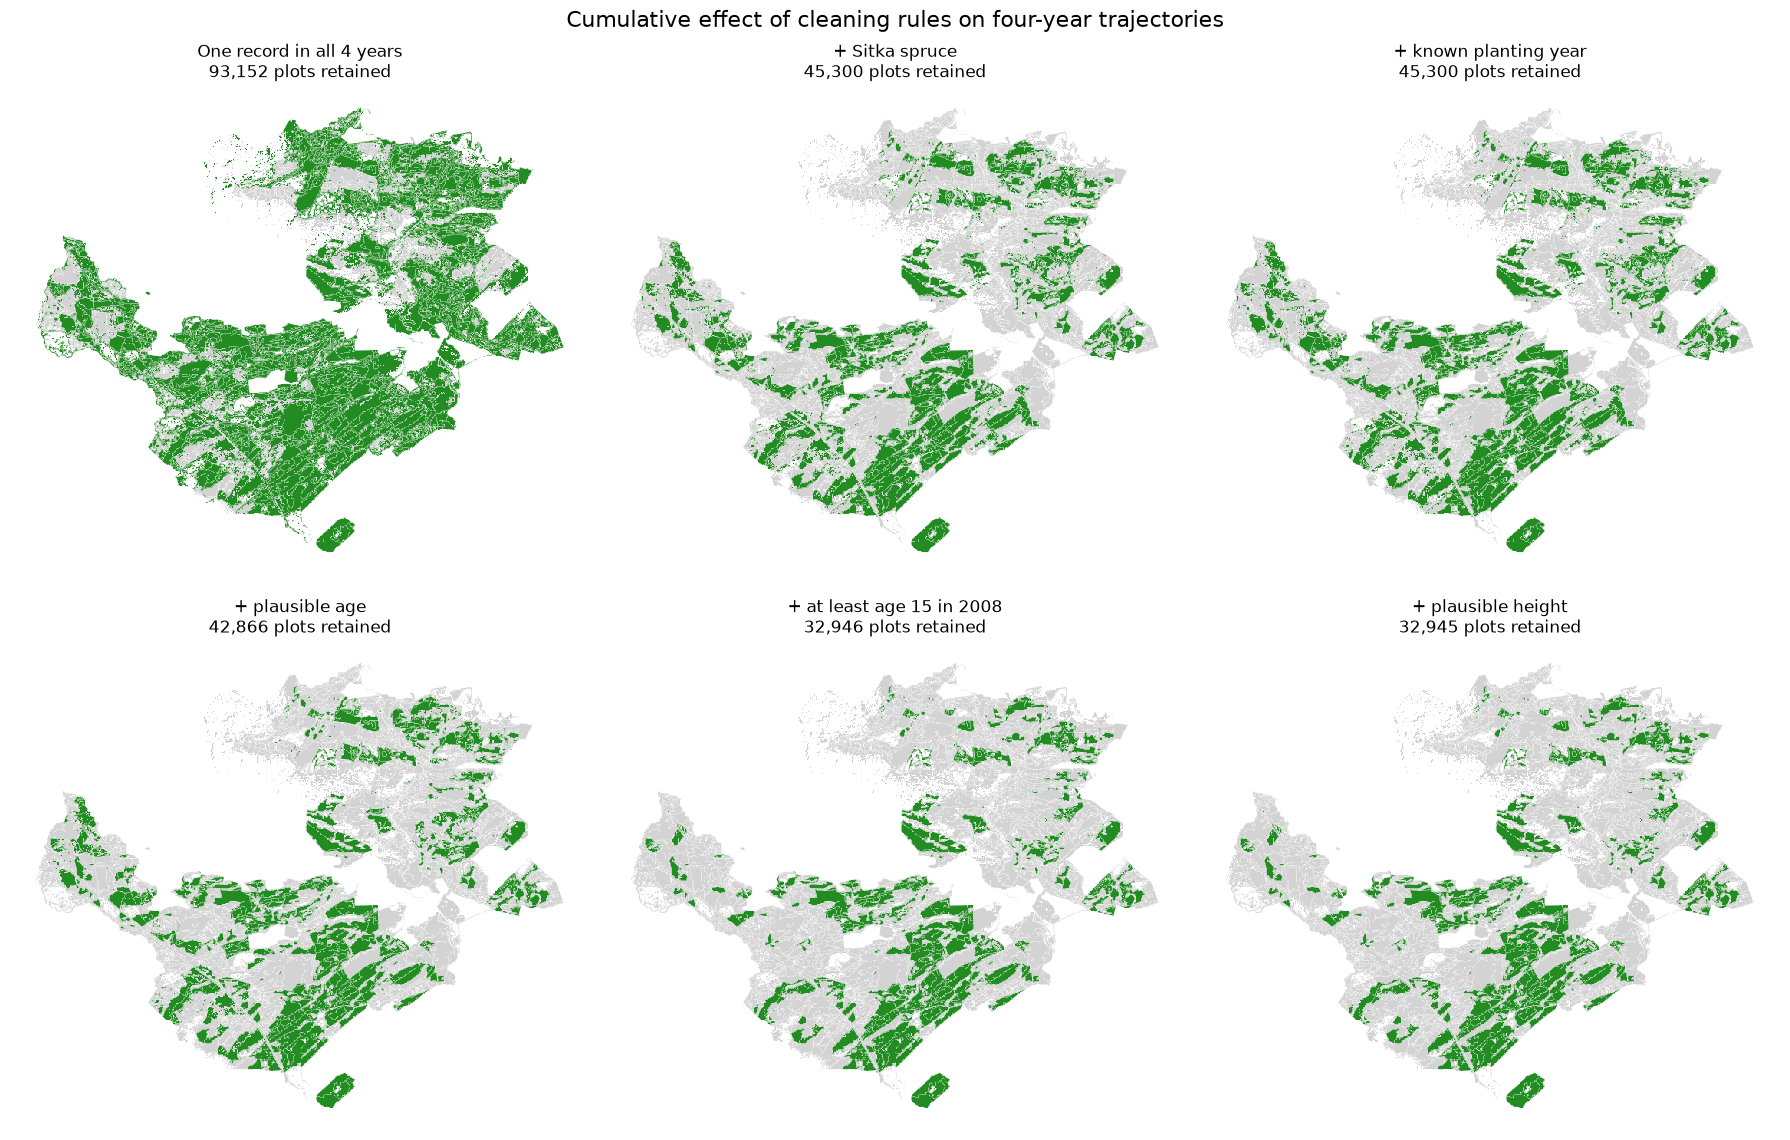
\includegraphics[width=\textwidth]{figures/legacy_examples/cleaning_stages_map_example.png}
\caption{Example figure from an earlier Aberfoyle dataset/workflow. Included to illustrate the planned analysis; not a final result. Cumulative spatial effect of the cleaning rules on an earlier four-year cohort extract (retained plots in green, removed in grey). Plot counts and geometry do not match the current cohorts in Table~\ref{tab:cohorts}.}
\label{fig:cleaning-stages}
\end{figure}

\section{Response variable and Chapman-Richards residuals}

The response is \texttt{Top\_Height95}. CR parameters ($y_{\max}$, $k$, $p$) are fitted once, by least squares, using \texttt{Age} as the time input across all plot-timestamp pairs. The residual for plot $i$ at time $t$ is
\[
\varepsilon_{i,t} = y_{i,t}^{\text{obs}} - y_{\text{CR}}(t_i \mid y_{\max}, k, p),
\]
where a positive value means the plot is taller than the age-matched CR baseline, and a negative value means shorter. This fit has not yet run on the current cohorts; Chapter~\ref{ch:results} reports placeholders until it does.

\section{Terrain, wind, climate, and soil data}

Terrain variables -- elevation, slope, northness, eastness, TWI, and TOPEX -- will come from the OS Terrain 50 DTM \citep{osdatahub2026OSTerrain50} (50\,m post spacing) at each plot centroid, using \texttt{rasterio} and \texttt{geopandas}. WASP wind data will be added if available with a documented resolution; otherwise the Global Wind Atlas \citep{globalwindatlas2026GlobalWindAtlas} (250\,m grid) serves as a public fallback, using the lowest above-ground height relevant to canopy exposure. None of this extraction has run yet.

HadUK-Grid \citep{hollis2019HadUKGridGriddedClimate} gives 1\,km gridded daily UK climate data, used for interval-level indices such as summer soil moisture deficit and growing degree days, one value per survey interval. At 1\,km it is coarse next to plot scale, so it is a temporal signal, not a spatial predictor, unless extraction shows real within-forest variation. Soil data is treated the same way: included only if it shows enough unique values inside Aberfoyle to distinguish nearby plots. Neither has been extracted yet.

\section{Leakage risks and excluded variables}
\label{sec:data-leakage}

Some GeoPackage fields are derived from height, age, or both, and would leak the target. These are excluded from all predictor sets: \texttt{Vol95}, \texttt{Vol99}, \texttt{Vol\_RM95} (from height, area, canopy cover), \texttt{GYCspec95} and \texttt{GYCspec99} (from height and age, with some infinite or extreme values), the raw height percentiles, and \texttt{Top\_Height99}.

\texttt{whcl} is a Forest Research windthrow hazard class, not a raw wind measurement, and looks management-linked: plots with \texttt{whcl > 4} are thinned in only 2.63\% of records (312 plots), and class 6 is almost entirely unthinned. It is kept for audit only.

Management fields (\texttt{Thin}, \texttt{last\_thinn}, \texttt{time\_since\_thinning}) are useful context but not a substitute for terrain and wind attribution: \texttt{Thin} only records whether a last-thinning year exists, not whether it affected the observed interval. Thinning is the main unobserved confounder, discussed further in Chapter~\ref{ch:discussion}.

\section{Multicollinearity}

A correlation matrix and variance inflation factor (VIF) check are planned before modelling, since elevation, TOPEX, and any wind layer likely overlap. Figure~\ref{fig:correlation-example} shows the intended format. XGBoost should handle correlated predictors implicitly; the linear baseline will drop the more redundant variable in pairs with VIF above 10.

\begin{figure}[h]
\centering
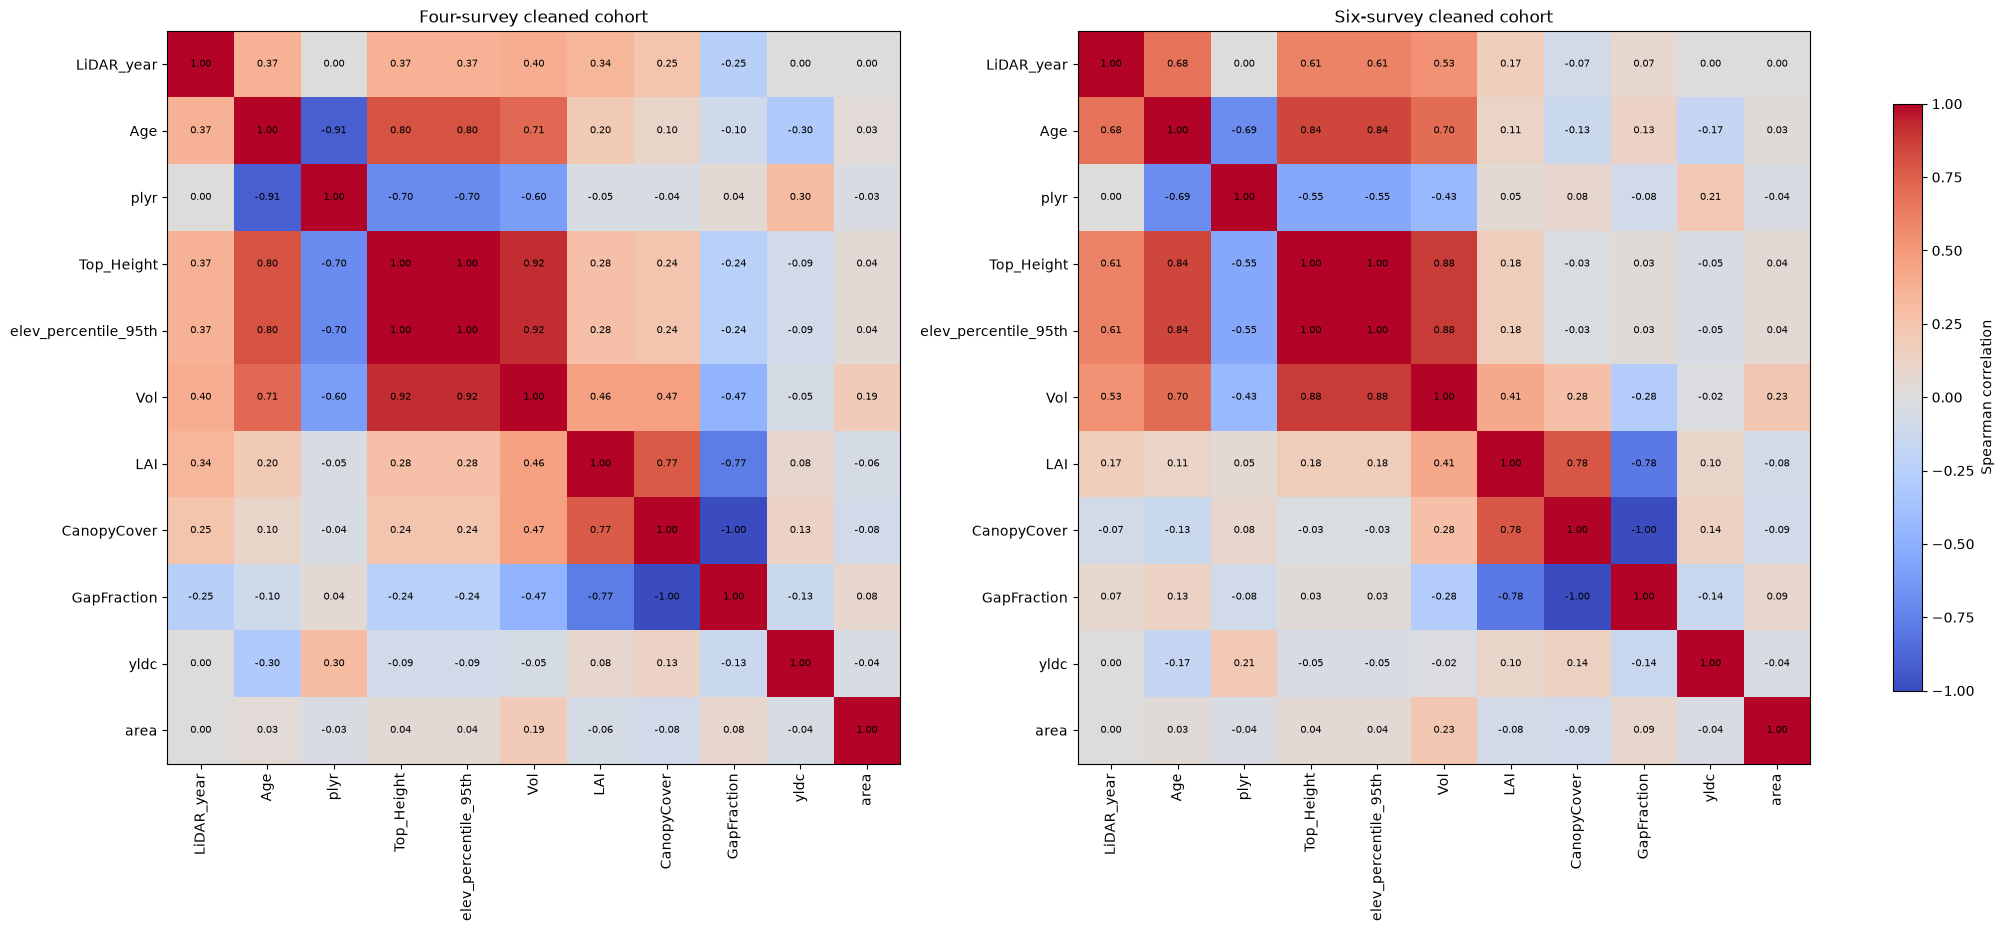
\includegraphics[width=\textwidth]{figures/legacy_examples/correlation_matrix_example.png}
\caption{Example figure from an earlier Aberfoyle dataset/workflow. Included to illustrate the planned analysis; not a final result. Spearman correlation matrix for the four-survey and six-survey cohorts from an earlier cleaning pass, before terrain and wind features were joined.}
\label{fig:correlation-example}
\end{figure}

\chapter{Methodology}
\label{ch:methodology}

The methodology goes from simplest to most complex. Each stage should give a result that stands on its own, so if later stages are not finished, earlier stages still answer part of the question.

\section{Overview: explaining the residual}

The core idea is simple. First, fit the Chapman-Richards curve using only \texttt{Age}. This curve is the biological baseline: it says how tall a plot should be, given its age, if every plot in Aberfoyle were the same. Subtracting this baseline from the observed height gives a residual for each plot and survey year. That residual is what \texttt{Age} alone cannot explain.

The rest of the methodology tries to explain that residual using terrain and wind variables. XGBoost and SHAP are used first, as an independent check on which variables matter. The Env-PINN then goes one step further: instead of only predicting the residual, it lets the growth ceiling $y_{\max}$ itself become a function of terrain and wind, so the model learns a different ceiling for each plot rather than one ceiling for the whole forest.

\section{Chapman-Richards baseline}

CR parameters ($y_{\max}$, $k$, $p$) are fitted once, by least squares, across all plot-timestamp pairs in the four-survey cohort. This single fit is the baseline every later model must beat, and it is also the source of the residuals used below.

\section{CR residuals and trajectory classification}

The residual $\varepsilon_{i,t}$ for each plot-timestamp pair is the observed height minus the CR-predicted height at that age. Plots with at least two timestamps get a mean residual $\bar{\varepsilon}_i$. Each plot is then classified into one of three groups: persistent under-performer ($\bar{\varepsilon}_i < -\delta$), CR-conformant ($|\bar{\varepsilon}_i| < \delta$), or persistent over-performer ($\bar{\varepsilon}_i > \delta$). The threshold $\delta$ is roughly 2\,m, tuned from the residual distribution rather than fixed in advance.

\section{Spatial residual analysis}

Global Moran's I \citep{moran1950NotesContinuousStochastic} is computed on $\bar{\varepsilon}_i$, using an 8-nearest-neighbour spatial weights matrix, to test whether over- and under-performing plots cluster or scatter at random. A significant positive result supports spatial attribution. A null result would not rule out terrain effects, but would shift more weight onto the feature-level results in Section~\ref{sec:methodology-xgb}. Local Moran's I (LISA) \citep{anselin1995LocalIndicatorsSpatial} then locates specific clusters.

\section{Train and test sets}
\label{sec:train-test}

Different models use different splits, and it matters which. The simple baselines (CR check, linear regression) and both PINN versions train on 2002--2012 and test on 2021 and 2023. The 2021--2023 interval is never seen during training, so it is a genuine test of whether the model generalises across the long 2012--2021 gap. XGBoost instead uses a spatial holdout split: whole regions are held out for testing rather than random rows, because random splits on spatially autocorrelated data place training and test points next to each other and can overstate accuracy \citep{roberts2017CrossvalidationStrategiesData}. The CR baseline fit itself (above) is not split into train and test; it is fitted once on the full cohort, since its role is to define the baseline curve, not to be evaluated as a predictor.

\section{Simple baselines}

Before any machine learning model, the CR model and a linear regression are both checked on the 2002--2012 / 2021--2023 split above. If these baselines behave oddly, for example if linear regression beats CR by a wide margin, the cleaning pipeline is revisited before moving on to XGBoost or the PINN.

\section{XGBoost and SHAP attribution}
\label{sec:methodology-xgb}

XGBoost \citep{chen2016XGBoostScalableTree} is fitted in up to three feature-set versions (Table~\ref{tab:xgb-versions}), using the spatial holdout split from Section~\ref{sec:train-test}.

\begin{table}[h]
\centering
\begin{tabular}{lll}
\toprule
Version & Features & Purpose \\
\midrule
XGB-A & Terrain only & What does terrain alone explain? \\
XGB-B & Terrain + WASP wind speed & Does measured wind add beyond TOPEX? \\
XGB-C & Terrain + Global Wind Atlas & Fallback if WASP is unavailable \\
\bottomrule
\end{tabular}
\caption{Planned XGBoost feature-set versions.}
\label{tab:xgb-versions}
\end{table}

SHAP values \citep{lundberg2017UnifiedApproachInterpreting}, via TreeSHAP \citep{lundberg2020LocalExplanationsGlobal}, rank feature importance for the richest available version, expected to be XGB-B. This ranking decides which features go into the Env-PINN sub-network, so SHAP runs before any PINN training.

\section{Baseline PINN (Version 1)}

The baseline PINN follows the standard formulation \citep{raissi2019PhysicsinformedNeuralNetworks}: a neural network branch and the CR branch run in parallel on the same age input, and the CR parameters stay frozen, so gradients only update the network. The physics loss compares derivatives, $d(\text{Height})/d(\text{Age})$, from the network against the same derivative from the CR equation, rather than comparing raw heights -- a stricter form of process-informed regularisation than a generic penalty on predicted values \citep{wesselkamp2024ProcessInformedNeuralNetworks}. The baseline PINN uses the split in Section~\ref{sec:train-test} and the single global $y_{\max}$, $k$, $p$ from the CR fit. It is the model every later version must improve on.

\section{Environmentally conditioned PINN (Env-PINN)}

The Env-PINN replaces the fixed global $y_{\max}$ with a learned function of environmental features $\mathbf{e}$:
\[
\hat{y}_{\max}(\mathbf{e}) = g_\phi(\mathbf{e}), \qquad g_\phi : \mathbb{R}^{n_e} \to \mathbb{R}_{>0}
\]
implemented as a small sub-network (two hidden layers of 32 units, ReLU, softplus output to keep $\hat{y}_{\max}$ positive). An anchor term, $\lambda_{\text{anc}} \cdot \frac{1}{N}\sum_i (\hat{y}_{\max}(\mathbf{e}_i) - \bar{y}_{\max})^2$, penalises large deviations from the mean learned ceiling, to stop the sub-network collapsing to a degenerate solution. It is pre-trained on XGB-B residuals before joint training, for stability. Two versions are planned: Version~2 uses terrain features only (elevation, TWI, TOPEX, northness, eastness); Version~3 uses the full SHAP-selected set, expected to include wind speed if it adds value.

\section{Ablation experiments}

Three ablations are planned once the Env-PINN trains: a sweep of the physics weight $\lambda_{\text{ph}}$ across six values, an anchor-strength ablation with $\lambda_{\text{anc}} \in \{0, 0.001, 0.1\}$ to check whether learned ceilings collapse without it, and a batch-size comparison (32 vs.\ 128).

\section{Convergent validity}

As a check, the Env-PINN sub-network's gradient sensitivity, $\partial \hat{y}_{\max} / \partial e_j$ for each feature $e_j$, is ranked and compared against the SHAP ranking from XGB-B using Spearman correlation. Agreement between two independently fitted methods is stronger evidence than either alone \citep{karniadakis2021PhysicsinformedMachineLearning, lundberg2017UnifiedApproachInterpreting}. Disagreement would not mean one method is wrong, but it would mean the attribution needs more caution before it is reported with confidence.

\chapter{Planned and Preliminary Results}
\label{ch:results}

This chapter is a draft. The terrain and wind extraction, the CR parameter fit on the current cleaned cohorts, and all model training described in Chapter~\ref{ch:methodology} have not been completed at the time of writing. The tables below are placeholders showing the intended reporting format. The figures are examples from an earlier version of the Aberfoyle dataset and workflow, included to show the type of output planned, not as final results.

\section{Trajectory analysis and spatial structure}

\subsection*{Chapman-Richards baseline fit}

Figure~\ref{fig:cr-example} shows the intended output format for the CR baseline: observed height-age trajectories for individual plots plotted against a fitted CR curve. The curve shown uses provisional parameters from an earlier exploratory pass and has not been refitted on the current cleaned four-survey cohort.

\begin{figure}[h]
\centering
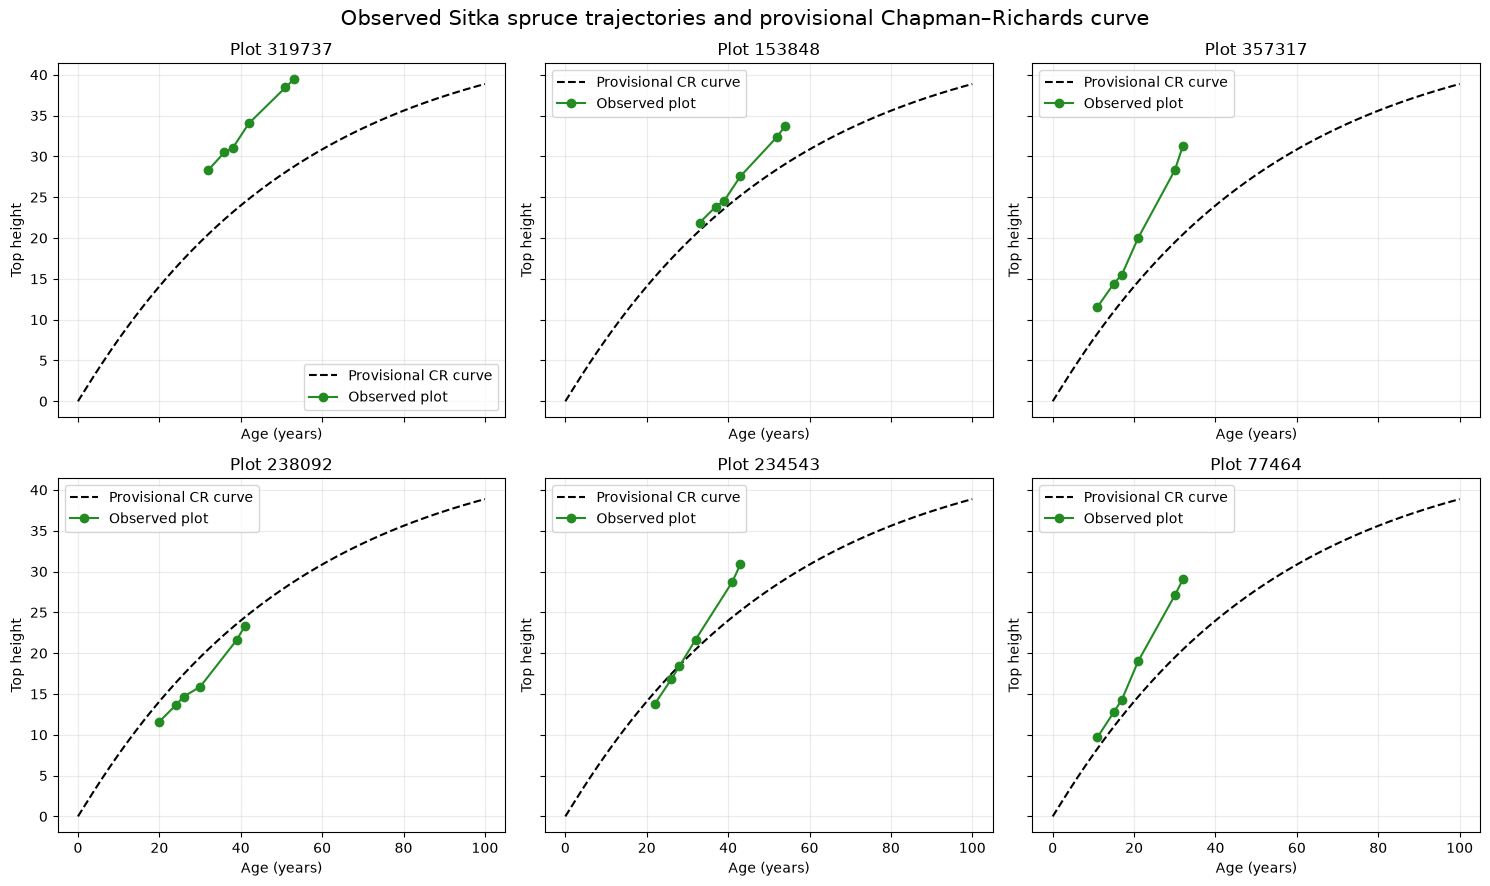
\includegraphics[width=\textwidth]{figures/legacy_examples/cr_trajectories_example.png}
\caption{Example figure from an earlier Aberfoyle dataset/workflow. Included to illustrate the planned analysis; not a final result. Observed Sitka spruce height-age trajectories for six example plots against a provisional Chapman-Richards curve fitted during exploratory analysis on a prior GeoPackage version.}
\label{fig:cr-example}
\end{figure}

\subsection*{Distribution checks by survey year}

Figure~\ref{fig:canopy-example} shows the intended format for checking whether a variable's distribution is stable or shifting across survey years, here for canopy cover on an earlier dataset version. The equivalent check for \texttt{Top\_Height95} on the current cleaned cohorts is outstanding.

\begin{figure}[h]
\centering
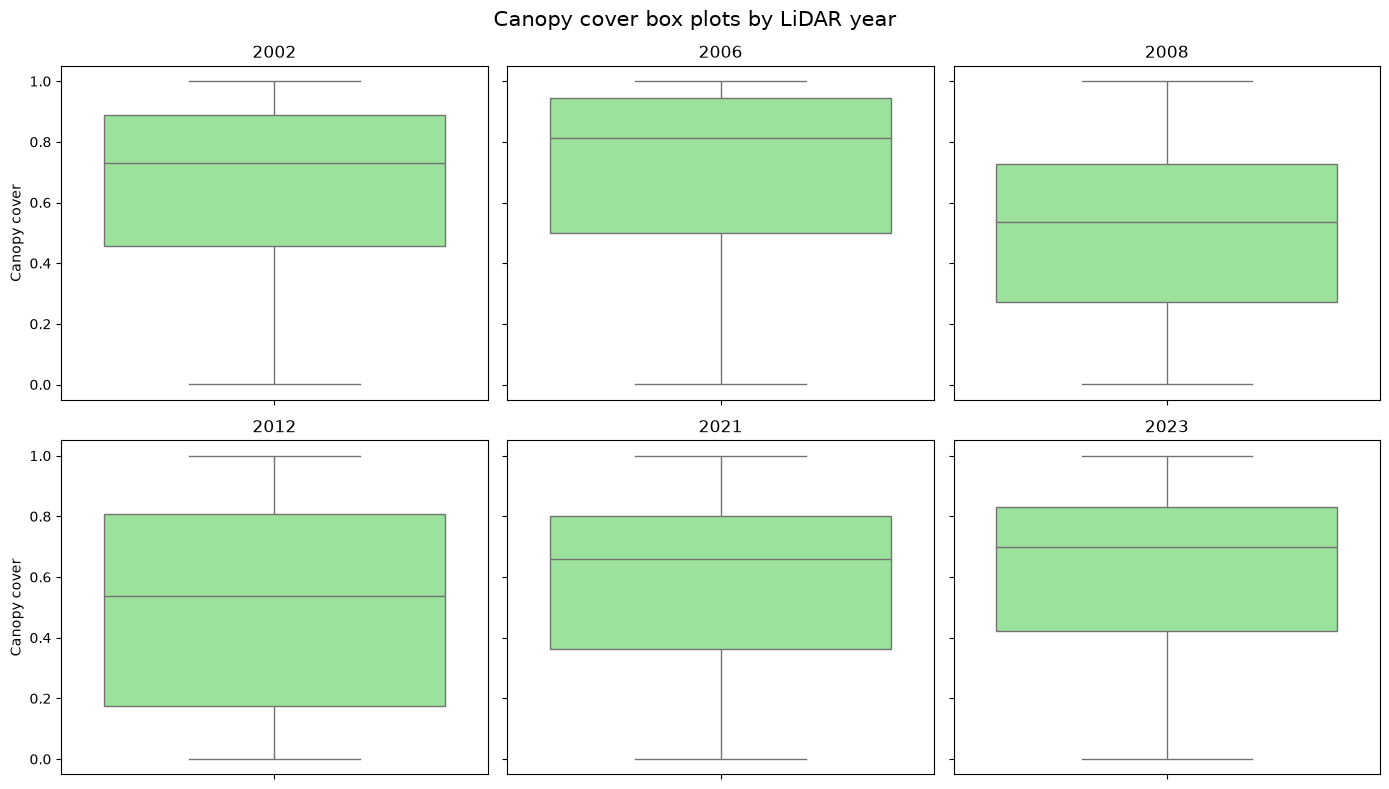
\includegraphics[width=\textwidth]{figures/legacy_examples/canopycover_by_year_example.png}
\caption{Example figure from an earlier Aberfoyle dataset/workflow. Included to illustrate the planned analysis; not a final result. Canopy cover box plots by LiDAR survey year, from an earlier exploratory pass on a prior GeoPackage version.}
\label{fig:canopy-example}
\end{figure}

\subsection*{Moran's I and trajectory classes}

\begin{table}[h]
\centering
\begin{tabular}{lc}
\toprule
Statistic & Value \\
\midrule
Global Moran's I on $\bar{\varepsilon}_i$ & TODO \\
$p$-value & TODO \\
Number of LISA high-high clusters & TODO \\
Number of LISA low-low clusters & TODO \\
\bottomrule
\end{tabular}
\caption{Placeholder: Moran's I and LISA results, not yet computed on the current cleaned cohort.}
\label{tab:moran-placeholder}
\end{table}

\section{Spatial attribution: XGBoost and SHAP}

\begin{table}[h]
\centering
\begin{tabular}{lccc}
\toprule
Model & RMSE & R\textsuperscript{2} & Top 3 SHAP features \\
\midrule
XGB-A (terrain only) & TODO & TODO & TODO \\
XGB-B (terrain + wind) & TODO & TODO & TODO \\
\bottomrule
\end{tabular}
\caption{Placeholder: XGBoost attribution results, pending terrain and wind feature extraction.}
\label{tab:xgb-placeholder}
\end{table}

\section{Env-PINN results}

\begin{table}[h]
\centering
\begin{tabular}{lccccc}
\toprule
Model & MAE & MSE & R\textsuperscript{2} & MRE & Accuracy \\
\midrule
CR (global parameters) & & & & & \\
Linear regression & & & & & \\
XGB-B (terrain + wind) & & & & & \\
PINN v1 (baseline, global $y_{\max}$) & & & & & \\
Env-PINN v2 (terrain-conditioned) & & & & & \\
Env-PINN v3 (full-conditioned) & & & & & \\
\bottomrule
\end{tabular}
\caption{Placeholder: model comparison table. To be reported separately for all plots, persistent under-performers, and CR-conformant plots once training is complete.}
\label{tab:model-comparison-placeholder}
\end{table}

\section{Synthesis (placeholder)}

Once the above results exist, this section will report what fraction of between-plot growth variation terrain and wind features explain (from the XGB-B $R^2$), whether Moran's I on the XGBoost residuals drops relative to Moran's I on the raw CR residuals (a check on whether the features genuinely capture spatial structure rather than simply proximity), and what fraction of variation remains unexplained -- expected, based on the data audit in Chapter~\ref{ch:data}, to include a contribution from unrecorded thinning and management events.

\chapter{Discussion}
\label{ch:discussion}

This chapter is written ahead of the results it discusses, since terrain and wind extraction and model training are not yet complete (Chapter~\ref{ch:results}). It sets out how the expected results should be read, and what they would not prove.

\section{What the expected results would mean}

If terrain and wind features explain a meaningful share of the CR residual variation, and the Env-PINN's learned $\hat{y}_{\max}(\mathbf{e})$ agrees with the independent SHAP ranking, that would be reasonable evidence that some of Aberfoyle's plot-to-plot growth variation is linked to terrain and exposure, not just noise. It would not prove that terrain \emph{causes} the difference, since the analysis is observational: terrain is not randomly assigned to plots, and it correlates with unmeasured factors such as land-use history.

\section{What attribution can and cannot prove}

A significant Moran's I result would show that residuals cluster spatially. It would not, on its own, separate a genuine terrain effect from a proximity effect, since neighbouring plots share many unmeasured traits beyond terrain. This is why Moran's I is also planned on the XGBoost residuals, not just the raw CR residuals: if clustering drops once terrain and wind are included, that better supports the features capturing real structure, rather than just standing in for proximity.

\section{Management and thinning as a confounder}

Thinning is the most likely source of misleading results here. The \texttt{Thin} field only records whether a last-thinning year exists, not whether it affected the observed growth interval, and windthrow hazard class correlates with thinning status in ways that suggest management is not independent of terrain (Chapter~\ref{ch:data}). A plot classed as a persistent over-performer could, in some cases, simply have been thinned in a way the data does not capture. This cannot be fixed with the current data. It is a boundary on how strongly the results can be read, and requesting fuller management records from Forest Research is the highest-value follow-up (Section~\ref{sec:future-work}).

\section{Limits from sparse timestamps and coarse climate data}

Six survey years, with a nine-year gap between 2012 and 2021, limits the temporal sub-question. HadUK-Grid climate indices are averaged across each gap, so a single index cannot tell a bad year followed by a good one apart from steady moderate conditions; any claim about which interval mattered most for growth is descriptive, not a controlled comparison. HadUK-Grid, at 1\,km, is also coarse next to plot scale and may smooth over local terrain-driven microclimate. This is why it is used for forest-wide temporal indices, not spatial predictors, and why soil data is included only if extraction shows it varies meaningfully within the forest.

\section{Practical value for a forest Digital Twin}

Even with these limits, a spatial map of learned growth ceilings has direct use: it can flag plots where the CR baseline is likely wrong before a manager relies on it, without resurveying every stand. That is narrower than a full Digital Twin, but it is the kind of attribution layer such a system would need, and it is deliverable from the current dataset regardless of what the temporal question finds.

\section{Future work}
\label{sec:future-work}

The single highest-value addition would be fuller thinning and felling records from Forest Research, so management events can be flagged directly rather than inferred from canopy cover and windthrow class. Three further extensions follow from the current design: replacing the CR physics loss with a process-based model such as 3-PG once monthly climate inputs are available; letting the growth-rate parameter $k$, not only $y_{\max}$, vary with interval-level climate; and running the Env-PINN forward under future climate scenarios once a suitable projection dataset is identified. None of these are part of the current scope.

\chapter{Conclusions}
\label{ch:conclusion}

This dissertation asks what environmental and terrain factors explain why some Sitka spruce plots in Aberfoyle grow faster or slower than the Chapman-Richards baseline predicts. The approach: compute CR residuals across a cleaned, balanced cohort of plots surveyed by airborne LiDAR at up to six timestamps between 2002 and 2023; test whether the residuals cluster spatially; identify which terrain and wind features best explain them using XGBoost and SHAP; then build a physics-informed neural network in which the growth ceiling $y_{\max}$ is learned from those same features instead of fixed globally.

At this draft stage, the cleaned cohorts, the leakage-aware variable set, and the modelling pipeline are defined (Chapter~\ref{ch:data}). Terrain and wind feature extraction, the CR fit on the current cohorts, and all downstream modelling are outstanding (Chapter~\ref{ch:results}). The dissertation will deliver: a spatial residual analysis with Moran's I and trajectory classification; an XGBoost and SHAP attribution comparing terrain-only and terrain-plus-wind feature sets; an Env-PINN with terrain-conditioned and fully-conditioned versions, evaluated against a baseline PINN and simpler baselines; an ablation study isolating what drives any improvement; and a convergent validity check between the Env-PINN's learned feature sensitivity and the SHAP ranking.

The intended contribution is a spatial map of learned growth ceilings across Aberfoyle, showing which parts of the forest are environmentally constrained and by how much. This is framed as attribution evidence, not as a causal or predictive claim beyond what the data and validation can support.

\chapter{Research Plan, Milestones, and Deliverables}
\label{ch:research-plan}

This chapter sets out the remaining work needed to complete the dissertation. It updates an earlier project-proposal planning section to the current growth-attribution scope; the earlier proposal covered a windthrow-classification project using NFI plots, AlphaEarth embeddings, and a Harwood Forest transfer test, none of which are part of this dissertation and none of which are carried forward here.

\section{Phase 1: Data verification and cleaning}

Verify the LiDAR-derived Aberfoyle plot data against Forest Research metadata where possible. Confirm the current GeoPackage (\texttt{LiDAR\_Years\_All\_7jul.gpkg}), the Sitka spruce layer, and the cleaned four-survey and six-survey cohorts described in Chapter~\ref{ch:data}. Confirm \texttt{Top\_Height95}, \texttt{Age}, \texttt{spis}, and the excluded leakage variables against the field documentation. Identify what metadata is still missing from Forest Research -- in particular, confirmation of the LiDAR acquisition platform and exact plot/grid-cell geometry.

\section{Phase 2: Spatial feature extraction}

Extract elevation, slope, aspect (as northness and eastness), TWI, and TOPEX from OS Terrain 50 or the best available DTM, at each plot centroid. Add WASP wind data if it becomes available with a documented resolution. Add Global Wind Atlas as a public fallback or comparison layer if WASP is unavailable or undocumented. Test whether HadUK-Grid or candidate soil datasets show meaningful within-forest variation before treating either as a spatial predictor, rather than assuming coarse products are unusable without checking.

\section{Phase 3: Baseline growth and residual analysis}

Fit the Chapman-Richards baseline using \texttt{Age} and \texttt{Top\_Height95} on the current cleaned cohorts. Compute CR residuals for every plot-timestamp pair. Map the residuals. Test spatial clustering using Moran's I and, if the result supports it, LISA. Classify plots into persistent under-performers, conformant plots, and over-performers.

\section{Phase 4: Interpretable attribution models}

Fit simple baselines (CR, linear regression) first, as a sanity check before any machine learning model. Fit XGBoost using terrain-only, terrain-plus-WASP, and terrain-plus-Global-Wind-Atlas feature sets where data availability allows. Use SHAP to identify the terrain and wind features that best explain growth residuals. Use spatial, not random-only, validation throughout.

\section{Phase 5: Env-PINN development}

Build the baseline CR-PINN (Section~\ref{ch:methodology}). Build the environmentally conditioned PINN in which $\hat{y}_{\max}(\mathbf{e})$ is learned from terrain and wind features. Run ablations for physics loss weight, anchor regularisation strength, and feature set. Compare the Env-PINN's feature sensitivity against the XGBoost SHAP ranking.

\section{Phase 6: Evaluation, discussion, and writing}

Compare CR, linear regression, XGBoost, the baseline PINN, and the Env-PINN on a consistent evaluation set. Evaluate whether terrain and wind features reduce residual spatial structure (Moran's I on model residuals versus raw CR residuals). State limitations clearly: sparse and unevenly spaced timestamps, management and thinning confounding, uncertain wind-data resolution, and coarse climate and soil products. Complete the dissertation write-up, figures, appendices, and bibliography.

\section{Deliverables}

\begin{itemize}
  \item Cleaned modelling cohort documentation (this draft, Chapter~\ref{ch:data}).
  \item Data audit table (Chapter~\ref{ch:data}; Appendix~\ref{app:data-dictionary}).
  \item Terrain and wind feature extraction table, once features are extracted.
  \item CR residual maps.
  \item Moran's I and LISA results.
  \item XGBoost and SHAP attribution results.
  \item Env-PINN model and ablation results.
  \item A learned spatial map of plot-level growth ceilings.
  \item The final dissertation draft.
  \item Reproducible code and notebooks, where practical, alongside the dissertation.
\end{itemize}

\section{Timeline}

Table~\ref{tab:timeline} gives an indicative weekly timeline for the remaining work. Timing is approximate and will be updated as data availability (particularly WASP wind data) and early model results become clear.

\begin{table}[h]
\centering
\begin{tabular}{cll}
\toprule
Weeks & Phase & Notes \\
\midrule
1--2 & Phase 1: Data verification & Confirm metadata gaps with Forest Research \\
2--4 & Phase 2: Spatial feature extraction & OS Terrain 50 first; WASP/GWA as available \\
4--6 & Phase 3: Baseline and residual analysis & CR fit, Moran's I, trajectory classes \\
6--9 & Phase 4: XGBoost + SHAP attribution & Feature ranking feeds into Phase 5 \\
9--13 & Phase 5: Env-PINN development & Baseline PINN, then Env-PINN v2/v3, ablations \\
13--15 & Phase 6: Evaluation and writing & Model comparison, discussion, final polish \\
\bottomrule
\end{tabular}
\caption{Planned dissertation workflow. Timing is indicative and will be updated as data availability and model results become clear.}
\label{tab:timeline}
\end{table}


\bibliographystyle{plainnat}
\bibliography{mybibfile}

\appendix
\chapter{Abbreviations}
\label{app:abbreviations}

\begin{table}[h]
\centering
\begin{tabular}{ll}
\toprule
Abbreviation & Expansion \\
\midrule
CR & Chapman-Richards \\
PINN & Physics-Informed Neural Network \\
Env-PINN & Environmentally conditioned PINN (this work) \\
TWI & Topographic Wetness Index \\
TOPEX & Topographic Exposure index (wind shelter) \\
SMD & Soil Moisture Deficit \\
PET & Potential Evapotranspiration \\
GDD & Growing Degree Days \\
SHAP & SHapley Additive exPlanations \\
WASP & Wind Atlas Analysis and Application Program \\
HadUK-Grid & Met Office 1\,km gridded UK climate observations \\
OS & Ordnance Survey \\
DT & Digital Twin \\
VIF & Variance Inflation Factor \\
LISA & Local Indicators of Spatial Association \\
\bottomrule
\end{tabular}
\caption{Abbreviations used in this dissertation.}
\end{table}

\chapter{Data Dictionary and Variable Exclusions}
\label{app:data-dictionary}

This appendix summarises the variable exclusions described in Section~\ref{sec:data-leakage}. It is a draft summary; the full field dictionary from Forest Research metadata is not yet reproduced here in full.

\begin{table}[h]
\centering
\begin{tabular}{lp{9cm}}
\toprule
Variable(s) & Reason excluded from top-height predictor sets \\
\midrule
\texttt{Vol95}, \texttt{Vol99}, \texttt{Vol\_RM95} & Derived from height, area, and canopy cover; would leak the height target. \\
\texttt{GYCspec95}, \texttt{GYCspec99} & Derived from height and age via a Chapman-Richards-style formula; also contain infinite/extreme values in places. \\
\texttt{elev\_percentile\_95th}, \texttt{elev\_percentile\_99th} & Direct raw inputs to \texttt{Top\_Height95}/\texttt{Top\_Height99}; using them would duplicate the target. \\
\texttt{Top\_Height99} & Alternative height outcome, not an independent predictor; also affected by the \texttt{Top\_Height99 < Top\_Height95} inconsistency. \\
\texttt{whcl} & Forest Research windthrow hazard class; management-linked, not a raw wind measurement. Retained for audit/stratification only. \\
\texttt{p1--p5}, \texttt{g1}, \texttt{g3} & Chapman-Richards and volume-equation lookup coefficients, not plot-level environmental predictors. \\
\texttt{Species}, \texttt{SPIS\_RF} & Disagree systematically with the inventory \texttt{spis} field used for Sitka spruce filtering. \\
\bottomrule
\end{tabular}
\caption{Summary of excluded variables and reasons.}
\end{table}

\chapter{Cleaning Audit}
\label{app:cleaning-audit}

The cleaning rules applied to produce the balanced Sitka spruce cohorts (Section~\ref{ch:data}) are, in order: keep the required cohort years; keep plots present in every required year; filter to Sitka spruce using \texttt{spis == "SS"}; keep valid planting years; keep plausible age (\texttt{Age = LiDAR\_year - plyr}); keep plausible \texttt{Top\_Height95} values. A plot failing any rule in any required year is removed entirely, so the retained cohort stays balanced across timestamps. Volume-based filtering is not applied as a general cleaning rule; negative \texttt{Vol\_RM95} values remain in the master export.

Outstanding audit questions to raise with Forest Research before final modelling: confirmation of the LiDAR acquisition platform; confirmation of exact plot/grid-cell geometry; and clarification of the \texttt{Top\_Height99 < Top\_Height95} inversion beyond the known multiplier effect.

\chapter{Mathematical Details}
\label{app:math-details}

\section{Chapman-Richards equation}

\[
y(t) = y_{\max} \left(1 - e^{-kt}\right)^{p}
\]

where $y(t)$ is height at age $t$, $y_{\max}$ is the asymptotic maximum height, $k$ controls the growth rate, and $p$ controls curve shape. Parameters are fitted by least squares across all plot-timestamp pairs (Section~\ref{ch:methodology}).

\section{Topographic Wetness Index (TWI)}

\[
\text{TWI} = \ln\left(\frac{A}{\tan \beta}\right)
\]

where $A$ is the upslope contributing area per unit contour length and $\beta$ is the local slope angle, both derived from the DTM. Higher TWI indicates greater expected soil water accumulation.

\section{TOPEX}

TOPEX is computed as the sum of angles to the horizon in a fixed set of compass directions (commonly eight), measured from the DTM at each point, giving a single index of topographic shelter versus exposure. Higher TOPEX values indicate more sheltered locations; lower (more negative) values indicate more exposed locations. The exact radius and direction count used for the Aberfoyle extraction is to be confirmed during Phase 2 (Chapter~\ref{ch:research-plan}).

\section{Env-PINN loss function}

\[
\mathcal{L}_{\text{total}} = \mathcal{L}_{\text{data}} + \lambda_{\text{ph}} \cdot \mathcal{L}_{\text{physics}}\big(\hat{y}_{\max}(\mathbf{e})\big) + \lambda_1 |\theta|_1 + \lambda_2 |\phi|_1 + \lambda_{\text{anc}} \cdot \frac{1}{N}\sum_i \big(\hat{y}_{\max}(\mathbf{e}_i) - \bar{y}_{\max}\big)^2
\]

where $\theta$ are the main network parameters, $\phi$ are the environmental sub-network parameters, $\mathcal{L}_{\text{physics}}$ compares network and CR derivatives with respect to age (Section~\ref{ch:methodology}), and the final anchor term regularises the learned growth ceiling toward the cohort mean $\bar{y}_{\max}$.

\chapter{Extra Figures}
\label{app:extra-figures}

Reserved for additional figures once terrain extraction and model training are complete: full (unclipped) SHAP spatial maps, Env-PINN training loss curves across ablation configurations, a high-resolution $\hat{y}_{\max}(\mathbf{e})$ surface, the full trajectory class map, and the full feature correlation matrix. None of these are available at the current draft stage.


\end{document}
